\chapter{Lecture 9: More Applications of Cauchy's theorem}

\section{The order of a zero of a function}

\begin{lemma}
    [Order of a zero of a function]
    Suppose $f$ is analytic in a disc $D$, $f$ is not identically zero, and $f(z_0) = 0$. Then for some $z_0$ in $D$, we have
    \begin{equation*}
        f(z) = \sum_{n=0}^{\infty} a_n(z - z_0)^n
    \end{equation*}
    Let $m \geq 1$ be the smallest $n \in \mathbb{Z}_{\geq 0}$ such that $a_n \neq 0$. That is:
    \begin{equation*}
        f(z) = a_m(z - z_0)^m + a_{m+1}(z - z_0)^{m+1} + \cdots
    \end{equation*}
    \underline{Say:} $f$ has a zero of order $m$ at $z_0$.
    Equivalently:
    \begin{equation*}
        f(z) = f^{\prime}(z_0) = f^{\prime\prime}(z_0) = \cdots = f^{(m-1)}(z_0) = 0 \label{eq:order_of_zero}
    \end{equation*}
    Yet $f^{(m)}(z_0) \neq 0$. \\
    \underline{Then} $g(z) = \frac{f(z)}{(z - z_0)^m}$ is analytic in $D$ and $g(z_0) \neq 0$.
    \underline{Since}
    \begin{equation*}
        g(z) = a_m + a_{m+1}(z - z_0) + \cdots
    \end{equation*}
    Converges because:
    \begin{equation*}
        (z - z_0)^m \left[ a_{m+1} + a_{m+2}(z - z_0) + \cdots \right] = f(z) - a_m(z - z_0)^m
    \end{equation*}
    Converges in $D$.

\end{lemma}

\begin{proof}
    This proof will demonstrate the conclusion of equation \ref{eq:order_of_zero}. \\
    \underline{Let} $f(z) = a_m(z - z_0)^m + a_{m+1}(z - z_0)^{m+1} + \cdots$ \\
    Notice that $(z - z_0) = 0$ at $z = z_0$. \\
    \underline{Thus:}
    \begin{align*}
        f^{\prime}(z)       & = m a_m(z - z_0)^{m-1} + (m+1)a_{m+1}(z - z_0)^m + \cdots = 0           \\
        f^{\prime\prime}(z) & = m(m-1)a_m(z - z_0)^{m-2} + (m+1)m a_{m+1}(z - z_0)^{m-1} + \cdots = 0 \\
                            & \vdots                                                                  \\
        f^{(m-1)}(z)        & = m! a_m(z - z_0) + m! a_{m+1}(z - z_0)^2 + \cdots = 0                  \\
        f^{(m)}(z)          & = m! a_{m}(z - z_0)^0 + m! a_{m+1}(z - z_0)^1 + \cdots \neq 0
    \end{align*}
\end{proof}

\section{A partial converse to the Cauchy integral formula}
\begin{theorem}
    [Morera's Theorem]
    if $f$ is continuous in a domain $D$ and
    \begin{equation*}
        \int_{\gamma} f(z) \, dz = 0
    \end{equation*}
    for every triangle $\gamma$ where $\gamma \in D$, and inside$(\gamma) \subseteq D$, $f$ is analytic in $D$.
\end{theorem}
\begin{proof}
    \begin{align*}
        \Omega                   & = \{|z-z_0| < r\} \quad r > 0 \quad r\text{ is small} \\
        \text{such that } \Omega & \in D                                                 \\
        \text{for } z            & \in \ \Omega \quad \text{we define}                   \\
        F(z)                     & = \int_{\gamma} f(\zeta) \, d\zeta,
    \end{align*}
    where the integral is taken along a radial curve
    \begin{figure}[H]
        \centering
        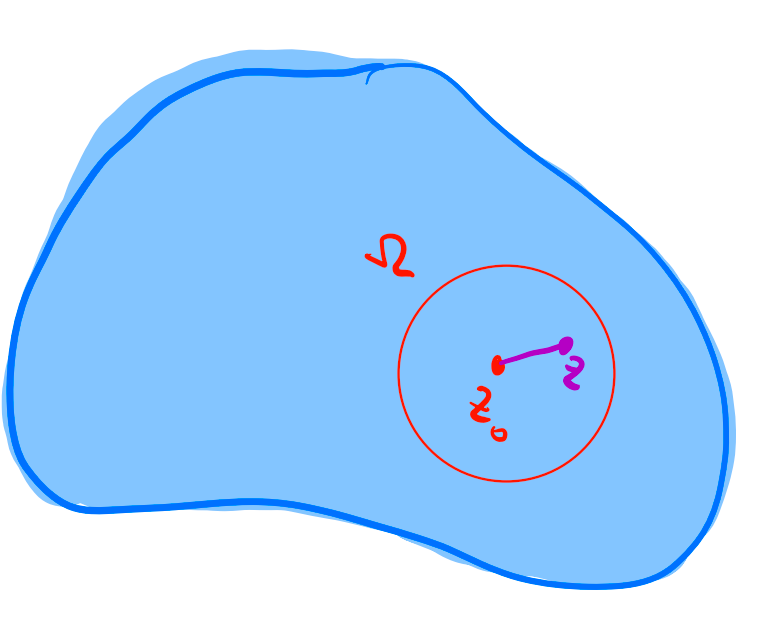
\includegraphics[width=0.4\textwidth]{./LECTURE_9/D.png}
        \caption{Radial curve}
        \label{fig:Radial curve}
    \end{figure}
    \textbf{\underline{Goal:}} F is analytic and F$^{\prime}(z) = f(z)$ (then it follows that $f$ is also analytic).
    \begin{equation*}
        F(z + h) - F(z) = \int_{z}^{z+h} f(\zeta) \, d\zeta
    \end{equation*}
    Since
    \begin{equation*}
        \int_{z_0}^{z} f(\zeta) \, d\zeta + \int_{z}^{z+h} f(\zeta) \, d\zeta - \int_{z_0}^{z+h} f(\zeta) \, d\zeta = 0
    \end{equation*}
    by assumption
    \begin{figure}[H]
        \centering
        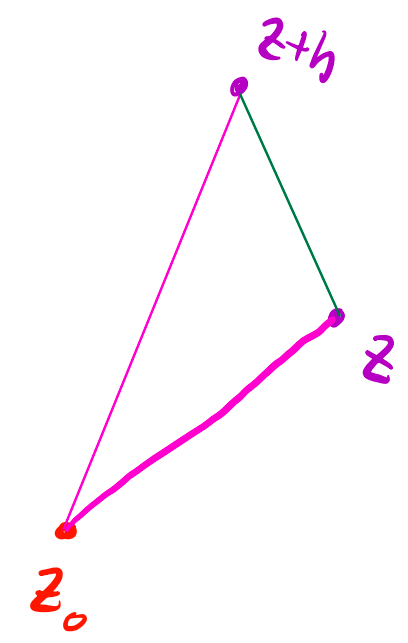
\includegraphics[width=0.4\textwidth]{./LECTURE_9/curve.png}
        \caption{Curve}
        \label{fig:Curve}
    \end{figure}
    \underline{\textbf{Thus:}}
    \begin{equation*}
        \frac{F(z+h) - F(z)}{h} - f(z) = \frac{1}{h} \int_{z}^{z+h} f(\zeta) - f(z)d\zeta
    \end{equation*}
    $\rightarrow$ This is because \begin{align*}
          & \int_{z}^{z+h} f(z)d\zeta \\
        = & f(z)\int_{z}^{z+h} d\zeta \\
        = & f(z) \cdot h
    \end{align*}
    By continuity of $f$, for any $\epsilon > 0$, there exists $\delta > 0$ such that $|f(w) - f(z)| < \epsilon$ if $|w - z| < \delta$.
    Then if $|h| < \delta$, we have:
    \begin{equation*}
        \left| \frac{F(z+h) - F(z)}{h} - f(z) \right| \leq \frac{1}{|h|} \epsilon |h| = \epsilon
    \end{equation*}
    Since $\epsilon$ is arbitrary, we have:
    \begin{equation*}
        \lim_{h \to 0} \frac{F(z+h) - F(z)}{h} = f(z)
    \end{equation*}
    \underline{\textbf{Thus:}} $F$ is analytic and $F^{\prime}(z) = f(z)$, as desired.
\end{proof}

\section{Applications}

\begin{theorem}
    [Liouville's Theorem]
    If $F$ is entire and $|F(z)| \leq M$ then $F$ is constant.
\end{theorem}

\begin{proof}
    \begin{align*}
        g(z)            & = \frac{F(z) - F(0)}{z} \quad \text{is entire since}                \\
        F(z)            & = F(0) + \sum_{n=1}^{\infty} a_n z^n                                \\
        \text{so } g(z) & = \sum_{n=1}^{\infty} a_n z^{n-1} = \sum_{n=0}^{\infty} a_{n+1} z^n
    \end{align*}
    Now
    \begin{equation*}
        |g(Re^{i\theta})| \leq \frac{|F(Re^{i\theta})| + |F(0)|}{R} \leq  \frac{2M}{R}
    \end{equation*}
    Using Cauchy's theorem, we have:
    \begin{align*}
        g(z_0) & = \frac{1}{2\pi} \int_{0}^{2\pi} \frac{g(z_0 + Re^{i\theta})}{Re^{i\theta}} \, iRe^{i\theta} \, d\theta \\
               & = \frac{1}{2\pi} \int_{0}^{2\pi} g(Re^{i\theta}) \, d\theta
    \end{align*}
    if $R >> |z_0|$, then $|z_0 + Re^{i\theta}| \geq R - |z_0|$
    \begin{figure}[H]
        \centering
        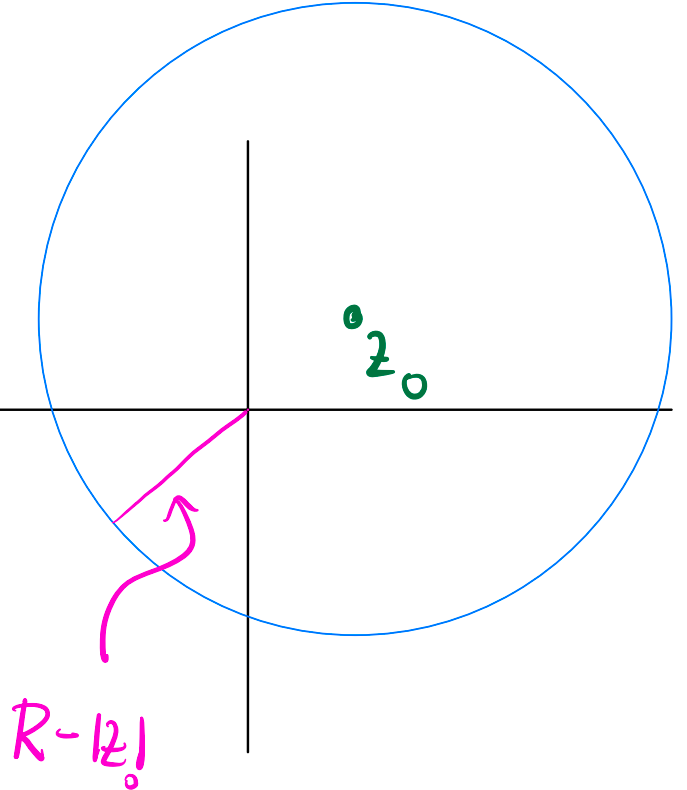
\includegraphics[width=0.4\textwidth]{./LECTURE_9/liouville.png}
        \caption{Circle}
        \label{fig:Circle}
    \end{figure}
    so
    \begin{equation*}
        |g(z_0)| \leq \frac{1}{2\pi} \int_0^{2\pi}|g(z_0 + Re^{i\theta})| \, d\theta \leq \frac{2M}{R-|z_0|}
    \end{equation*}
    But $R >> |z_0|$ is arbitrary, so taking $R \to \infty$ yields $g(z_0) = 0$ for all $z_0$ and $F(z_0) = F(0)$.
\end{proof}

\section{Analytic Logarithms}

\begin{lemma}
    [The logarithmic derivative]
    Let $D$ be a simply connected domain. \\
    Suppose $f$ is analytic in $D$ and $f \neq 0$ anywhere in $D$. \\
    Then $\frac{f^{\prime}}{f}$ is analytic in $D$ and hence so let's define:
    \begin{equation*}
        h^{\prime}(z) = \frac{f^{\prime}(z)}{f(z)}
    \end{equation*}
    Using the fundamental theorem of calculus, we have:
    \begin{equation*}
        h(z) = \int_{z_0}^{z} \frac{f^{\prime}(\zeta)}{f(\zeta)} \, d\zeta
    \end{equation*}
    Cauchy's theorem implies that $h(z)$ is analytic in $D$. \\
    Morera's theorem ensures that the integral can be taken over any path from $z_0$ to $z$ in $D$ and thus, $h(z)$ is path independent. \\
    So:
    \begin{align*}
        \left[e^{-h(z)}f(z)\right]^{\prime} & = -e^{-h(z)}h^{\prime}(z)f(z) + e^{-h(z)}f^{\prime}(z)              \\
                                            & = -e^{-h(z)}\frac{f^{\prime}(z)}{f(z)}f(z) + e^{-h(z)}f^{\prime}(z) \\
                                            & = 0
    \end{align*}
    So $e^{-h(z)}f(z) = f(z_0)$ is a constant. Or:
    \begin{align*}
        e^{-h(z)}f(z) & = f(z_0) \\
        f(z) = f(z_0)e^{h(z)}
    \end{align*}
    Thus $g (z) = h(z) + \text{Log}(f(z_0))$ satisfies:
    \begin{equation*}
        \begin{cases}
            e^{g(z)} = f(z) \\
            g(z) \quad \text{ is analytic in } D
        \end{cases}
    \end{equation*}
\end{lemma}

\section{Isolated Singularities}

\begin{definition}
    [Isolated Singularities]
    An analytic function has an \underline{isolated singularity at $z_0$} if it is analytic in a punctured disc $\{0 < |z - z_0| < r\}$ for some $r > 0$.
\end{definition}

\begin{example}
    $f(z) = \frac{z^2 - z_0^2}{z - z_0}$\\
    In this case $|f(z)|$ is bounded as $z \to z_0$. \\
    in fact, $f(z) = z + z_0$ ($z \neq z_0$) and $f$ can be extended to an analytic function at $z_0$.\\
    \underline{Thus:} $z_0$ is a \textbf{removable} singularity.
\end{example}

\begin{example}
    $f(z) = \frac{1}{(z - z_0)^4}$ \\

    $|f(z)| = \frac{1}{|z - z_0|^4} \to +\infty$ as $z \to z_0$.\\
    This is an example of a pole.
\end{example}

\begin{example}
    $f(z) = e^{\frac{1}{z - z_0}}$ \\

    $z_0 = 0$ for simplicity. \\
    $|f(z)| = e^{\frac{1}{2z} + \frac{1}{2\overline{z}}} = e^{\frac{x}{x^2 + y^2}}$ \\

    \begin{enumerate}
        \item If $y = 0$ and $x \to 0$ from $x > 0$, then $|f(z)| \to +\infty$.
        \item If $y = 0$ and $x \to 0$ from $x < 0$, then $|f(z)| \to 0$.
        \item If $x = 0$ and $y \to 0$ then $|f(z)| \to 1$, this is an \textbf{essential} singularity.
    \end{enumerate}
\end{example}

\section{Removable Singularities}

\begin{example}
    [Removable Singularity]
    Suppose $|f(z)|$ is bounded near $z_0$. \\
    Let
    \begin{equation*}
        g(z) = \begin{cases}
            (z-z_0)^2 f(z) & z \neq z_0 \\
            0              & z = z_0
        \end{cases}
    \end{equation*}
    \underline{Then}, $g(z)$ is analytic on $\{|z-z_0| < r\}$ for some $r > 0$. \\

    \underline{Since}\\
    \begin{equation*}
        \frac{g(z) - g(z_0)}{z - z_0} = (z - z_0)f(z)
    \end{equation*}
    \underline{and}
    \begin{equation*}
        \lim_{z \to z_0} (z - z_0)f(z) = 0
    \end{equation*}
    so $g'(z_0) = 0$ and thus:
    \begin{equation*}
        g(z)  = a_2(z-z_0)^2 + a_3(z-z_0)^3 + \cdots
    \end{equation*}
    \underline{So:}
    \begin{equation*}
        f(z) = \frac{g(z)}{(z-z_0)^2} = a_2 + a_3(z-z_0) + \cdots
    \end{equation*}
    If we set $f(z_0) = a_2$, then $f$ is analytic on $\{|z - z_0| < r\}$ and, we have \underline{\textbf{removed}} the singularity.
\end{example}

\begin{definition}
    $z_0$ is a \underline{removable singularity} of $f$ is bounded in a neighborhood of $z_0$.
\end{definition}

\section{Poles}

\begin{remark}
    Recall: if $f$ is analytic on $\{0 < |z - z_0| < R \}$ and $\lim_{z \to z_0} f(z) = \infty$, then $z_0$ is a pole of $f$.
\end{remark}

\begin{lemma}
    [Poles]
    Choose $r < R$ small enough that $|f(z)| > 1$ on $\{0 < |z-z_0| < r \}$. \\
    \underline{Then}: $g(z) = \frac{1}{f(z)}$ is analytic on $\{0 < |z - z_0| < r\}$ and $g(z) \to 0$ as $z \to z_0$. \\
    Thus, $g$ has a removable singularity and $g(z_0) = 0$.\\
    $z_0$ is a zero of order $m \geq 1$
    \begin{equation*}
        g(z) = (z - z_0)^m h(z)
    \end{equation*}
    where $h(z)$ is analytic and $h(z_0) \neq 0$ on $\{|z - z_0| < r\}$. \\
    \underline{Then}
    \begin{equation*}
        f(z) = \frac{1}{g(z)} = \frac{1}{(z - z_0)^m} \cdot \frac{1}{h(z)} = \frac{H(z)}{(z - z_0)^m}
    \end{equation*}
    Where $H(z)$ is analytic on $\{|z-z_0| < r\}$ and $H(z_0) \neq 0$.
\end{lemma}

\begin{definition}
    if $f(z) = \frac{H(z)}{(z - z_0)^m}$, where $H(z)$ is analytic on $\{|z - z_0| < r\}$ and $H(z_0) \neq 0$, then we say $f(z)$ has a pole of order $m$ at $z_0$.
\end{definition}

\section{Essential Singularities}

\begin{remark}
    Recall $f(z) = e^{\frac{1}{z}}$ has an essential singularity at $z = 0$. The behavior near essential singularities is wild.
\end{remark}

\begin{proposition}
    if $f$ is analytic on $\{0 < |z - z_0| < r\}$, with an essential singularity at $z_0$, then for any $w \in \mathbb{C}$, and any $\delta > 0, \exists z_\delta$ such that $0 < |z - z_0|< r$ and $|f(z) - w| < \delta$.
\end{proposition}
